%!TEX root = ED_Grafo.tex

\section{Análise de Circuitos Elétricos}
\begin{frame}[label=notas]
	A análise de circuitos elétricos com vários componentes passa pela construção
	de um sistema de equações lineares.
	\vfill
	Para análise utiliza-se: 
	\begin{itemize}
		\item as equações básicas dos componentes
		\item as leis de Kirchoff
	\end{itemize}
\end{frame}

\subsection{Leis de Kirchoff}
\begin{frame}[label=notas]
	\begin{block}{Lei das Correntes ou Leis dos Nós}
		Em um nó, a soma das correntes elétricas que entram é igual à soma das 
		correntes que saem, ou seja, um nó não acumula carga.
	\end{block}
	\begin{center}
		
\includegraphics[width=.3\textwidth]{Kirchhoff_current}\\%
		$i_1+i_4=i_2+i_3$
	\end{center}
\end{frame}

\begin{frame}[label=notas]
	\begin{block}{Lei das Tensões ou Lei das Malhas}
		A soma algébrica da diferença de potencial elétrico em um percurso 
		fechado é nula.
	\end{block}
	\begin{center}
		
\includegraphics[width=.4\textwidth]{Kirchhoff_voltage}\\%
		$v_1+v_2+v_3-v_4=0$
	\end{center}
\end{frame}

\newlength{\componentLength}\setlength{\componentLength}{15mm}%
\newlength{\wireOffset}\setlength{\wireOffset}{5mm}%
\newlength{\componentFullLength}\setlength{\componentFullLength}{\componentLength}%
\addtolength{\componentFullLength}{2\wireOffset}%
\newcommand{\componentH}[2]{%
	\draw (#2) -- ++(\wireOffset,0);
    \draw[decorate, decoration={#1}] ($(#2)+(\wireOffset,0)$) -- ++(\componentLength,0);
    \draw ($(#2)+(\wireOffset,0)+(\componentLength,0)$) -- ++(\wireOffset,0);
}%
\newcommand{\componentV}[2]{%
	\draw (#2) -- ++(0,\wireOffset);
    \draw[decorate, decoration={#1}] ($(#2)+(0,\wireOffset)$) -- ++(0,\componentLength);
    \draw ($(#2)+(0,\wireOffset)+(0,\componentLength)$) -- ++(0,\wireOffset);
}%
\newcommand{\drawCircuitCoords}{%
	\coordinate (c0) at(0,0);
	\coordinate (c1) at(0,\componentFullLength);
	\coordinate (c2) at(\componentFullLength,\componentFullLength);
	\coordinate (c3) at(2\componentFullLength,\componentFullLength);
	\coordinate (c4) at(2\componentFullLength,0);
	\coordinate (c5) at(\componentFullLength,\componentFullLength);
}%

\newcommand{\drawCircuit}[1][1-]{%
	\drawCircuitCoords%
	\uncover<#1>{
	\componentV{cell}{c0}%
    \componentH{resistor}{c1}%
    \componentH{inductor,amplitude=0.35cm, segment length=.5\componentLength}{c2}%
	\componentV{capacitor}{c4}%
    \draw (c3) -- ++(.5\componentFullLength,0);
	\componentV{resistor}{2.5\componentFullLength,0}%
    \draw (2.5\componentFullLength,0) -- (0,0);%
    }%
}%

\newcommand{\drawCircuitGraph}[1][1-]{%
	\drawCircuitCoords%
	\uncover<#1>{
    \foreach \x in {1,...,4}
		\node[draw,circle] (n\x) at(c\x) {C\x};
	\draw[->] (n1) -- (n2);
	\draw[->] (n2) -- (n3);
	\draw[->] (n3) -- (n4);
	\draw[->] (n4) -- (c0) -- (n1);
	\draw[->] (n3) -- ++(.5\componentFullLength,0) -- ++(0,-\componentFullLength) -- (n4);
	}%
}%

\begin{frame}[label=notas]
\begin{tikzpicture}[line width=1pt]
    \drawCircuit%
\end{tikzpicture}
\vfill
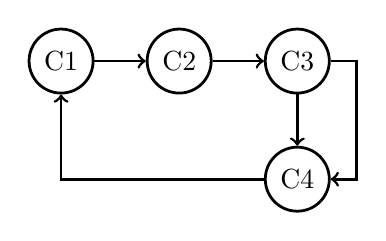
\begin{tikzpicture}[line width=1pt]
    \drawCircuitGraph[2]%
\end{tikzpicture}
\pause
\end{frame}
% Kirchhoff_voltage
% 
% 
% Kirchhoff's circuit laws are two equalities that deal with the conservation of charge and energy in electrical circuits, and were first described in 1845 by Gustav Kirchhoff.[1] Widely used in electrical engineering, they are also called Kirchhoff's rules or simply Kirchhoff's laws (see also Kirchhoff's laws for other meanings of that term).

% Both circuit rules can be directly derived from Maxwell's equations, but Kirchhoff preceded Maxwell and instead generalized work by Georg Ohm.